\section{Overview} \label{sec:overview}

This section first compares two prior systems and \parrot using
an example (\S\ref{sec:example}), and then describes \parrot's architecture
(\S\ref{sec:arch}).

\subsection{An Example} \label{sec:example}

%% TODO: switch to use latex listings
\begin{figure}[t]
\centering
\begin{minipage}{.5\textwidth}
\lgrindfile{parrot/code/example.cpp.lineno}
\end{minipage}
\vspace{-.1in}
\caption{{\em Simplified \pbzip.} It uses the producer-consumer idiom to
  compress a file in parallel.} \label{fig:example}
\vspace{-.05in}
\end{figure}

\begin{figure}[t]
\centering
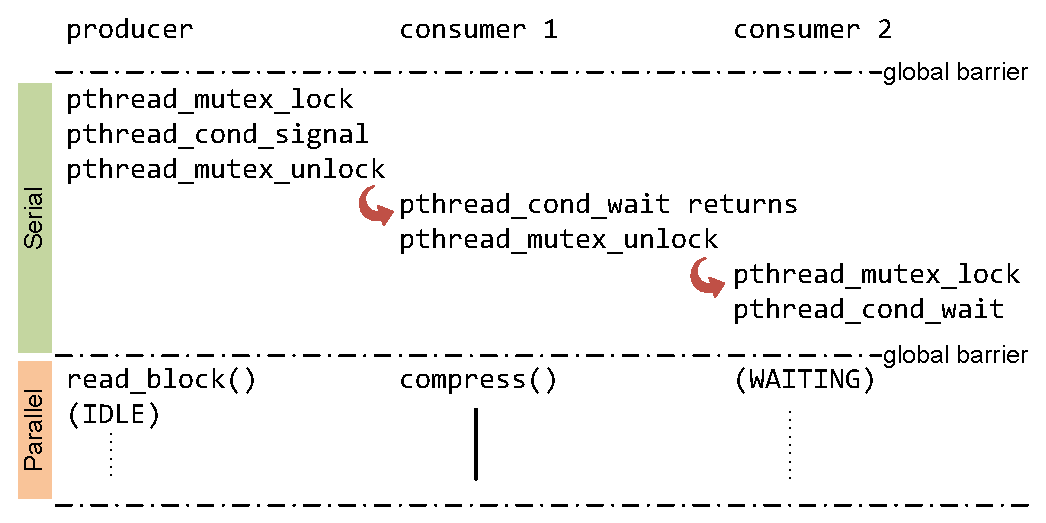
\includegraphics[width=\columnwidth]{parrot/figures/dthreads_schedule}
\vspace{-.2in}
\caption{{\em A \dthreads schedule.}  All
  \v{compress} calls are serialized. \v{read\_block} runs much faster than
  \v{compress}.}\label{fig:dthreads-schedule}
\vspace{-.05in}
\end{figure}

\begin{figure}[t]
\centering
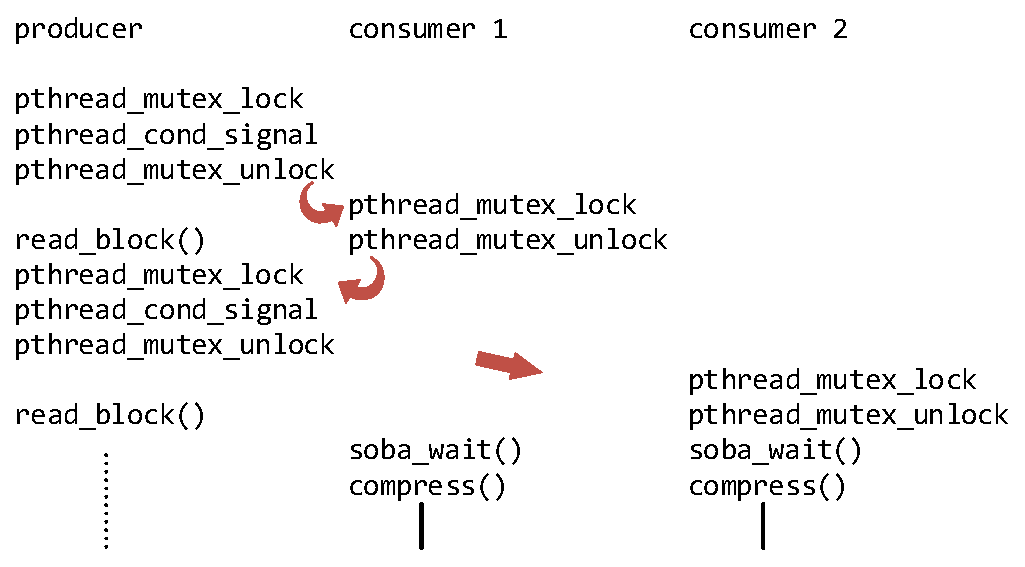
\includegraphics[width=\columnwidth]{parrot/figures/parrot_schedule}
\vspace{-.2in}
\caption{{\em A \parrot schedule with performance
    hints.}}\label{fig:parrot-schedule}
\vspace{-.05in}
\end{figure}

%% In this subsection, we present an example, explain why two prior systems
%% perform poorly on it, and illustrate how \parrot works with it.

Figure~\ref{fig:example} shows the example, a simplified version of the parallel
compression utility \pbzip\cite{pbzip2}.  It uses the common producer-consumer idiom:
the producer (main) thread reads file blocks, and multiple consumer
threads compress them in parallel.  Once the number of threads and the
number of blocks are given, one synchronization schedule suffices to
compress \emph{any} file, regardless of file content or size.  Thus, this program appears
easy to make deterministic and stable.  However, prior systems suffer from
various problems doing so, illustrated below using
two representative, open-source systems.
%% prior systems, chosen because they represent typical DMT or \smt
%% approaches and are open source.

%% \footnote{We used the example instead of the real \pbzip because we could
%%   not manage to make \pbzip work with the systems; see~$\S$\ref{sec:eval}.}

\coredet~\cite{coredet:asplos10} represents DMT systems that balance load
by counting instructions each thread has run~\cite{coredet:asplos10,
 kendo:asplos09, dmp:asplos09, dos:osdi10, ddos:asplos13}.  While the
schedules computed may have reasonable overhead, minor input or program
changes perturb the instruction counts and subsequently the schedules,
destabilizing program behaviors.  When running the example
with \coredet on eight different files, we observed
five different synchronization schedules.  This instability is
counterintuitive and raises new reliability challenges.  For instance,
testing one input provides little assurance for very similar inputs.
Reproducing a bug may require every bit of the bug-inducing input,
including the data a user typed, environment variables, shared libraries,
\etc. Missing one bit may deterministically hide the bug.  \coredet also
relies on static analysis to detect and count shared memory load and store
instructions, but the inherent imprecision of static analysis causes it to
instrument unnecessary accesses, resulting in high overhead.  On this
example, \coredet causes a 4.2$\times$ slowdown over nondeterministic execution with a 400
MB file and 16 threads.

% \footnote{Line XXX performs the \pbzip compression functionality
% and the intput filesize $n$ is equally split for $4$ consumer threads where
% $n=4, 32, 100, 400, 800, 1k, 4k, 8k$ bytes. We condfigure \coredet 
% in ownership tracking with 64-byte granularity and a quantum 
% size of $200k$ instructions.}
%% We also observed that adding \v{printf} statements led to different
%% schedules.  This instability is counterintuitive at least, and raises new
%% reliability challenges.  For instance, testing one input provides little
%% assurance on very similar inputs.  Reproducing a bug requires every bit of
%% the bug-inducing input, including not only the data a user typed, but also
%% environment variables, shared libraries, \etc.  A single missed bit may
%% deterministically hide the bug.  We observed 4.2x slowdown over
%% nondeterministic execution with a 400 MB file and 16 threads.  The reason
%% is that \coredet statically instruments shared memory loads and stores to
%% count instructions and make data races deterministic.  However, it is a
%% known-difficult problem to statically detect which memory locations may be
%% shared, so \coredet has to conservatively instrument many loads and stores,
%% causing unnecessary overhead.

%% The performance of \coredet on this example depends on the number of threads
%% and the size of inputfile where the later one dominates.
%% By choosing a $400k$ input file with 4 threads, \coredet gives more than
%% $60\%$ overhead while $400$\v{M} file gives 3$\times$ to 4$\times$ slowdown.
%% The performance yields more than 5$\times$ slowdown when we use more than
%% 16 threads.

\dthreads~\cite{dthreads:sosp11} represents \smt systems that
ignore load imbalance among threads.  It works by
alternating between a serial and a parallel phase, separated by global
barriers.  In a serial phase, it lets each thread do one synchronization in
order.  In a parallel phase, it lets threads run until all of them are about
to do synchronizations.  A parallel phase lasts as long as the slowest
thread, and is oblivious to the execution times of the other threads.  When
running the example with two threads, we observed the \dthreads schedule
in Figure~\ref{fig:dthreads-schedule}.  This schedule is stable because it
can compress any file, but it is also very slow because it serializes all
\v{compress} calls.  We observed \dthreadsexampleoverhead slowdown
with 16 threads; and more threads give bigger slowdowns.

This \emph{serialization} problem is not specific to only
\dthreads. Rather, it is general to all \smt systems that ignore load
imbalance.

%% make
%% schedules oblivious to computations but also unrealistically assume that
%% the schedules align with computations.  It works by alternating between a
%% serial and a parallel phase, separated by global barriers.  In serial
%% phase, it lets each thread do one synchronization in order.  In parallel
%% phase, it lets threads run until all of them are about to do
%% synchronizations.  This phase lasts as long as the slowest thread, and is
%% oblivious to the execution times of the other thread.  When running the
%% example with two threads, we observed the \dthreads schedule in
%% Figure~\ref{fig:dthreads-schedule}.  This schedule is stable because it
%% can compress any file, but it is also very slow because it serializes
%% all \v{compress} calls.  We observed 7.7x slowdown with 16 threads; more
%% threads give bigger slowdowns.

%% in which threads compute
%% locally and a serial phase in which threads do synchronizations in order.
%% The phases are separated by global barriers.


%% Its schedule are thus 
%% The parallel phase lasts as long as the slowest thread
%% Its schedule is thus oblivious to the local compute time of each thread.
%% can thus process a wide range of input because it is oblivious to how long
%% each thread computes in the parallel phases.
%% However, by ignoring compute
%% time, it can also lead to serious performance overhead.  

%%  which \emph{serialized} all calls to
%% \v{compress}, yielding the slowdown proporitonal to the the number of
%% threads; 16 threads gives more than 10$\times$ slowdown.

%% \peregrine~\cite{peregrine:sosp11} represents \smt systems that make
%% schedules oblivious to computations by recording and reusing schedules.
%% Recording can be slow; we observed XXX times slowdown when running the
%% example with \peregrine.  Moreover, to reuse a schedule, \peregrine requires
%% sophisticated program analysis to compute the constraints the schedule
%% places on inputs.


Running the example with \parrot is easy; users do
\vspace{-2 mm}
\begin{small}
\begin{verbatim}
$ LD_PRELOAD=./parrot.so program args...
\end{verbatim}
\end{small}
\vspace{-2 mm}

%, shown in Figure~\ref{fig:schedule} actually 
% more than 10 times slowdown when the number of threads is more than 16.

\noindent
During the execution, \parrot intercepts \pthread synchronizations.  Without
the hints at lines 3 and 23, \parrot schedules the synchronizations using round-robin. 
This schedule also serializes the \v{compress} calls, yielding the same slowdown as \dthreads.
Developers can easily detect this performance problem with
sample runs, and \parrot simplifies performance debugging by
deterministically reproducing the problem and reporting synchronizations
excessively delayed  by round-robin
(\eg, the return of \v{pthread\_cond\_wait} here).
%  When running the examplewith \parrot on a 400 MB file, we frequently
%  observed over 4s round-robin delay on \v{pthread\_mutex\_lock} in the
%  main thread.

To solve the serialization problem, we added a \compute at lines 3 and 23.  Line 3
informs \parrot that the program has a coscheduling group involving
\v{nthreads} threads, and line 23 is the starting point of coscheduling.  With
these hints, \parrot switched to the schedule in
Figure~\ref{fig:parrot-schedule} which ran \v{compress} in parallel,
achieving 0.8\% overhead compared to nondeterministic execution. A soft barrier is
different from classic synchronizations and can be safely 
ignored without affecting correctness.  For
instance, if the file blocks cannot be evenly divided among
the threads, the soft barrier will time out on the last round of input blocks.  Moreover,
for reasonable performance, we need to align only time-consuming computations
(\eg, \v{compress}, not \v{read\_block}).

%% Note that these hints need not be 100\% accurate because \parrot can time out
%% them without losing determinism.  Moreover, these hints need not align the
%% computation perfectly for reasonable performance.

% lasts longer than 4 seconds
%% Once developers discover this serialization, they can add \compute hints
%% (lines XX and XX) to let \parrot switch to a faster schedule that makes
%% \v{compress} calls run in parallel. In our sample run, the wait time of
%% \v{pthread\_mutex\_lock} in main thread lasts longer than 4 seconds when
%% the input file size is 400MB, which indicates a serializtion problem only
%% utilizes one thread and starves the rest.  Lines XXX and XXX show the
%% hints. Line XXX informs \parrot the size of the parallel computation group.
%% Line XXX informs \parrot the beginning point of a computation.  With the
%% hints, \parrot achieved comparable performance ($<$1\% overhead) to
%% nondeterministic execution.

%% To further help developers, \parrot also logs the wait
%% time of each synchronization for developers to identify excessive delays.

\begin{figure}[t]
\centering
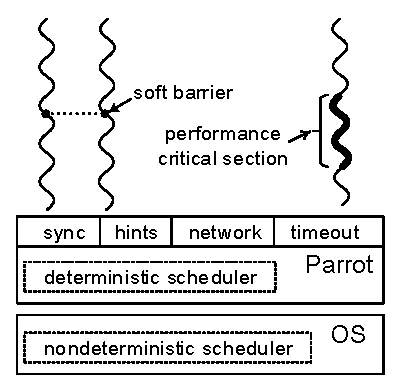
\includegraphics[width=.28\textwidth]{parrot/figures/architect}
%arch:
%programs with threads
%  computation  nondet regions
%      \  /
%       \/
%sync, hints, network, timeout, 
%deterministic scheduler, 
%OS schedule
\vspace{-.05in}
\caption{{\em \parrot architecture.}} \label{fig:arch}
\vspace{-.05in}
\end{figure}

\subsection{Architecture} \label{sec:arch}

Figure~\ref{fig:arch} shows \parrot's architecture.  We designed \parrot to be
simple and deployable.  It consists of a deterministic user-space
scheduler, implementation of hints, a set of wrapper functions for
intercepting \pthread, network, and timeout operations.  For simplicity,
the scheduler schedules only synchronizations, and delegates everything
else, such as assigning threads to CPU cores, to the OS scheduler.
The wrapper functions typically call into the scheduler for round-robin scheduling,
then delegate the actual implementation to \pthread or the OS.
Synchronizations in performance critical sections and inherently
nondeterministic operations (\eg, \v{recv}) are scheduled by the OS
scheduler.
